本章的“子工作组”部分,我们描述了集合功能以及集合功能如何表达公共通信模式。我们特别讨论了广播集合功能,它用于将值从组中的一个工作项传递到组中的其他工作项。本节介绍其他集合函数。\par

虽然本节中描述的集合函数,可以在程序中使用原子、工作组本地内存和栅栏等特性直接实现,但许多设备包括专用硬件对集合函数进行了加速。即使设备不包括专门的硬件,供应商提供的集合函数的实现可能针对它们的设备进行调优,因此调用内置集合函数通常会比编写的通用实现执行得更好。\par

\begin{tcolorbox}[colback=red!5!white,colframe=red!75!black]
为公共通信模式使用集合函数来简化代码并提高性能!
\end{tcolorbox}

工作组和子工作组都支持许多集合功能。其他集合功能仅支持子工作组\par

\hspace*{\fill} \par %插入空行
\textbf{广播}

广播功能允许组中的一个工作项与组中其他工作项共享变量的值。广播功能的工作原理如图9-12所示。工作组和子工作组都支持广播功能。\par

\hspace*{\fill} \par %插入空行
\textbf{投票}

any\_of和all\_of功能(今后将共同称为“投票”功能)使组内工作项比较的结果为一个布尔值:至少一个工作项的条件为真时,any\_of返回true;只有在所有工作项的条件为真时,all\_of返回true。对于一个输入示例,这两个函数的比较如图9-15所示。\par

\hspace*{\fill} \par %插入空行
图9-15 比较any\_of函数和all\_of函数
\begin{center}
	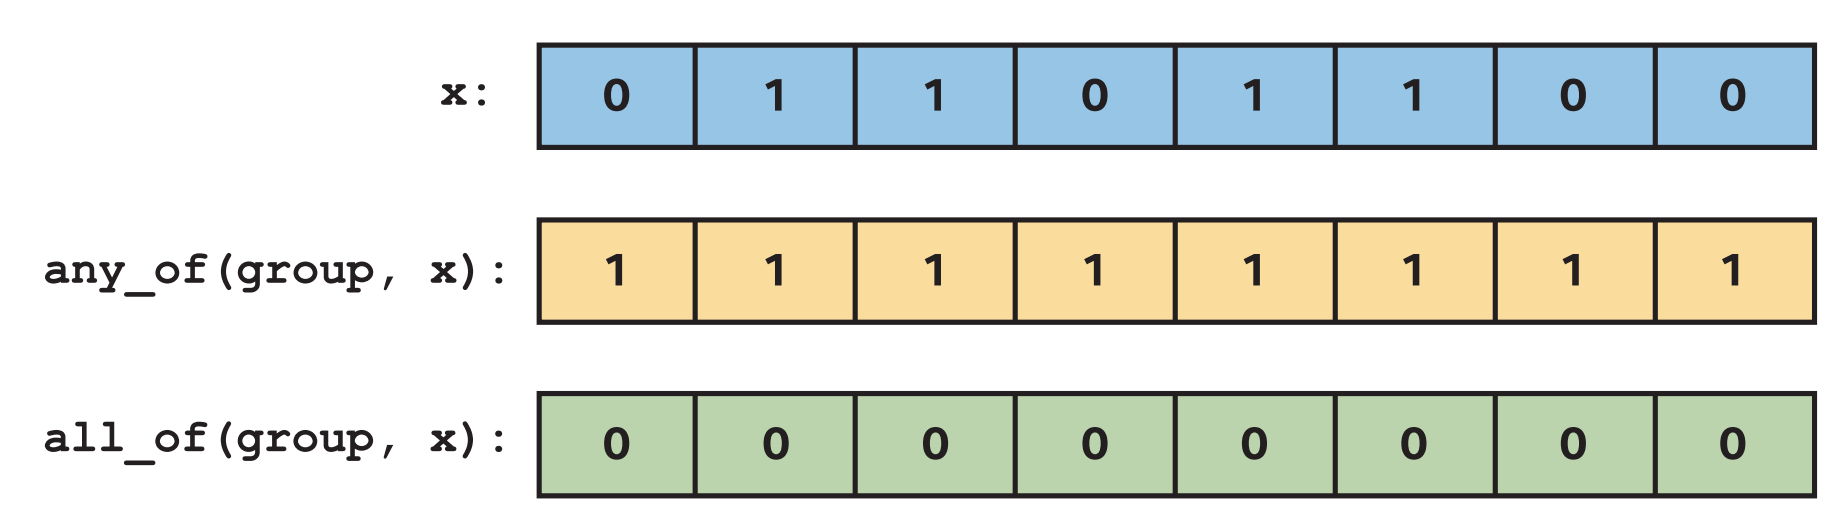
\includegraphics[width=1.\textwidth]{content/chapter-9/images/8}
\end{center}

工作组和子工作组都支持any\_of和all\_of投票函数。\par

\hspace*{\fill} \par %插入空行
\textbf{打乱}

子工作组最有用的特性之一是能够在单个工作项之间直接通信,而不需要显式的内存操作。许多情况下,例如:子工作组矩阵乘法内核,这些打乱操作使我们能够从内核中删除工作组本地内存的使用和/或避免对全局内存不必要的重复访问。这些打乱函数有几种类型。\par

最通用的打乱函数,称为shuffle,如图9-16所示,它允许子工作组中的任何工作项之间进行通信。然而,这种通用性可能会以性能为代价,我们强烈鼓励尽可能使用更特化的shuffle函数。\par

图9-16中,使用shuffle对预先计算的置换索引对子组的x值进行排序。展示了子工作组中一个工作项的箭头,其中shuffle的结果是local\_id等于7的工作项的x值。\par

\hspace*{\fill} \par %插入空行
图9-16 使用shuffle对预先计算的排列索引对x值排序
\begin{center}
	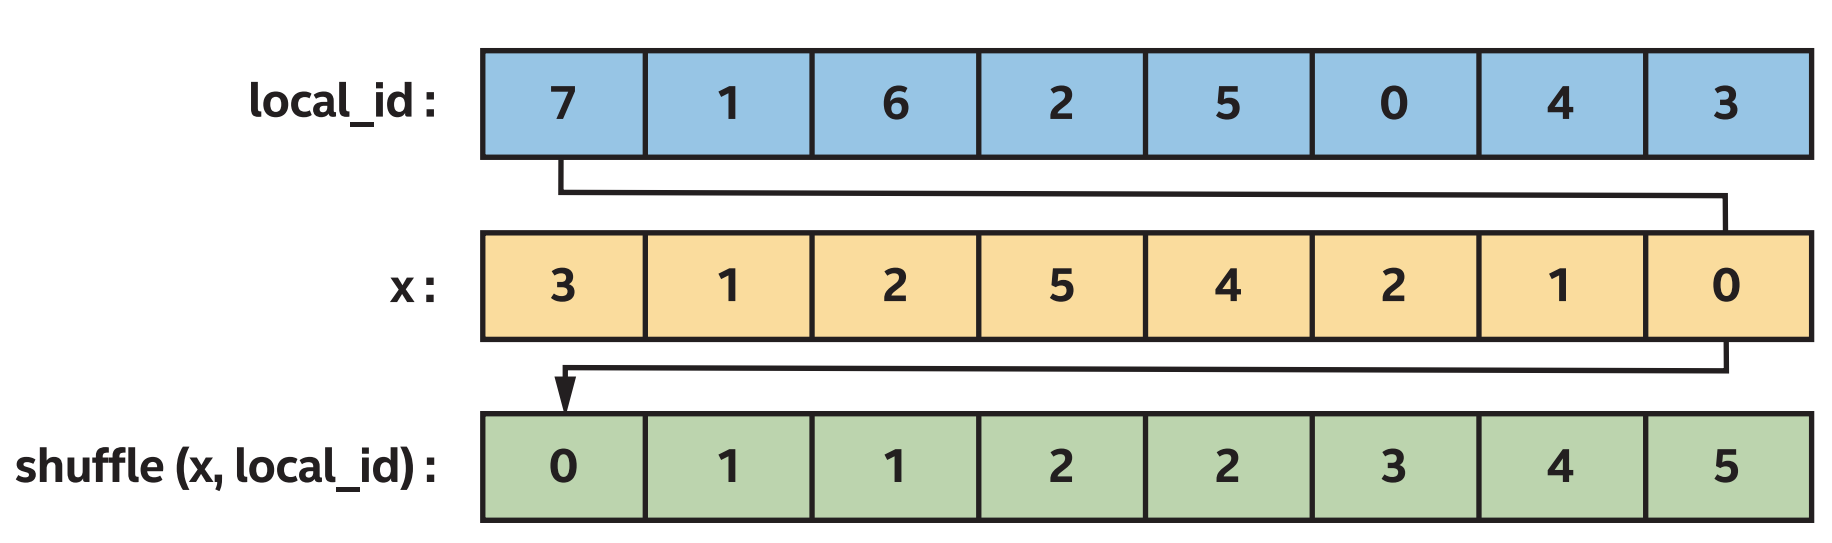
\includegraphics[width=1.\textwidth]{content/chapter-9/images/9}
\end{center}

注意,可以将子工作组广播函数视为shuffle的特化版,其中shuffle索引对于子工作组中的所有工作项是相同的,使用广播而不是shuffle可为编译器提供信息,并可能提高某些实现的性能。\par

shuffle\_up和shuffle\_down函数有效地将子工作组的内容向给定方向移动一定数量元素的长度,如图9-17所示。注意,返回到子工作组中最后五个工作项的值是未定义的,并且在图9-17中显示为空白。对于并行化带有循环依赖的循环,或者在实现扫描等常见算法时,移位非常有用。\par

\hspace*{\fill} \par %插入空行
图9-17 使用shuffle\_down将子组的x值移动5个元素的长度
\begin{center}
	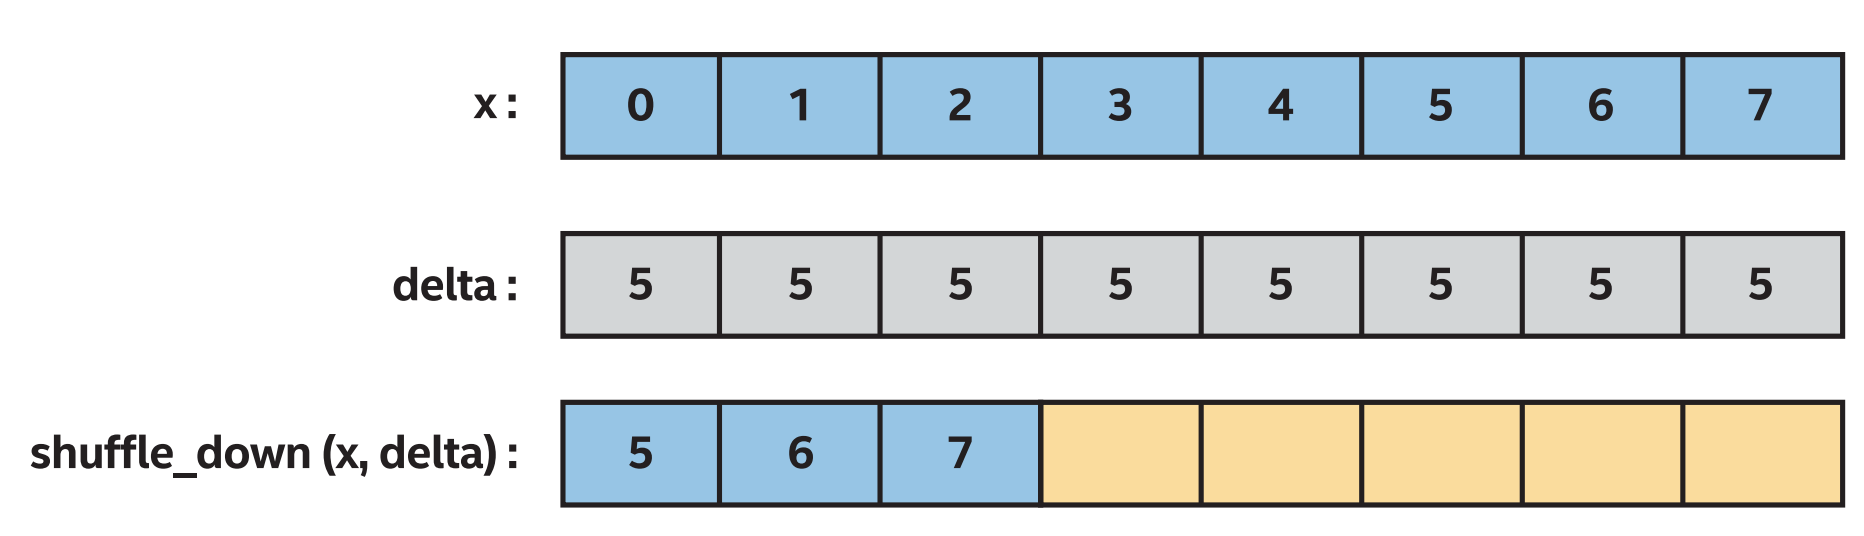
\includegraphics[width=1.\textwidth]{content/chapter-9/images/10}
\end{center}

shuffle\_xor函数交换两个工作项的值,这些值由应用于工作项的子工作组本地id和常量的XOR操作结果的的指定。如图9-18和9-19所示,几种常见的通信模式可以用异或表示,例如:交换相邻值对。\par

\hspace*{\fill} \par %插入空行
图9-18 使用shuffle\_xor交换相邻的x对
\begin{center}
	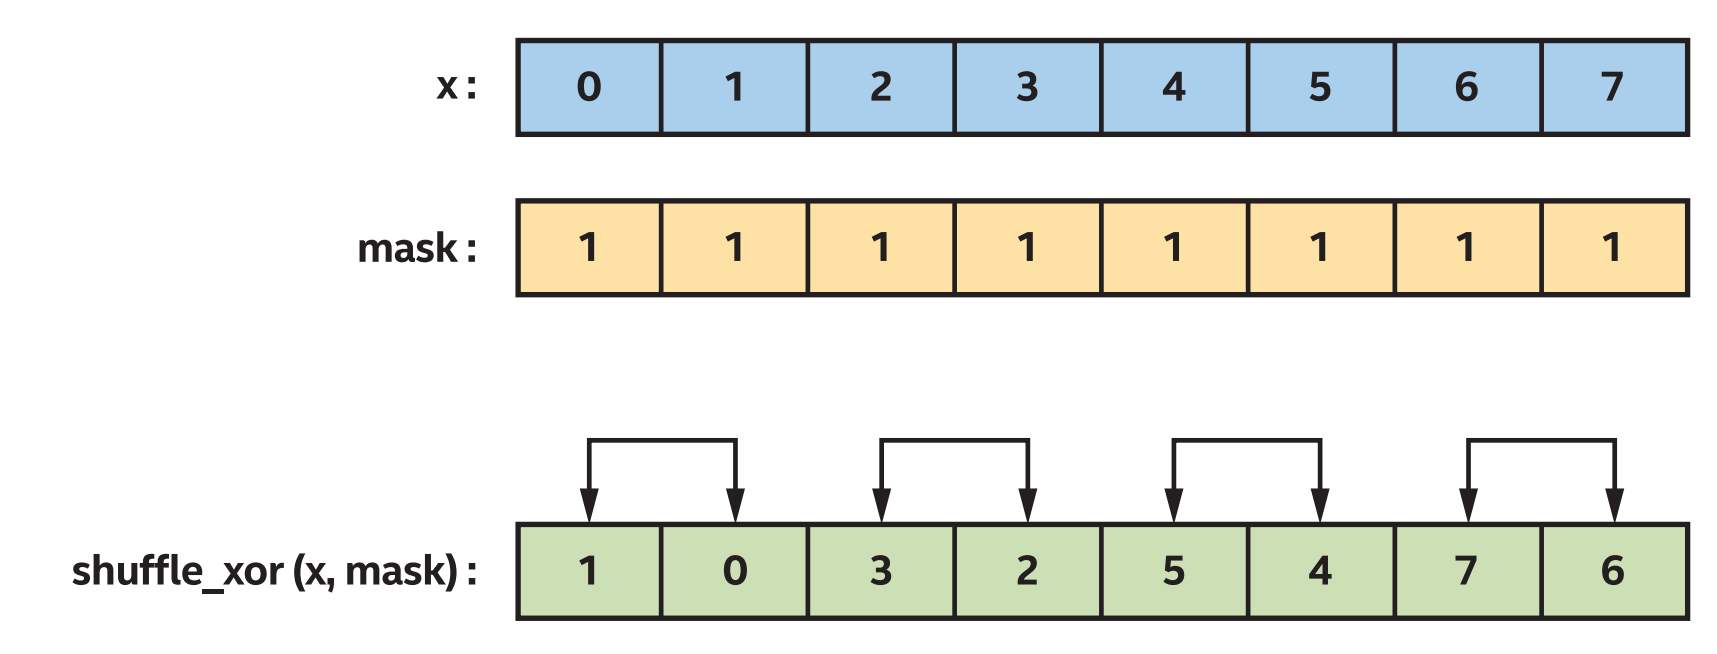
\includegraphics[width=1.\textwidth]{content/chapter-9/images/11}
\end{center}

或者反转子工作组的结果。\par

\hspace*{\fill} \par %插入空行
图9-19 使用shuffle\_xor反转x的值
\begin{center}
	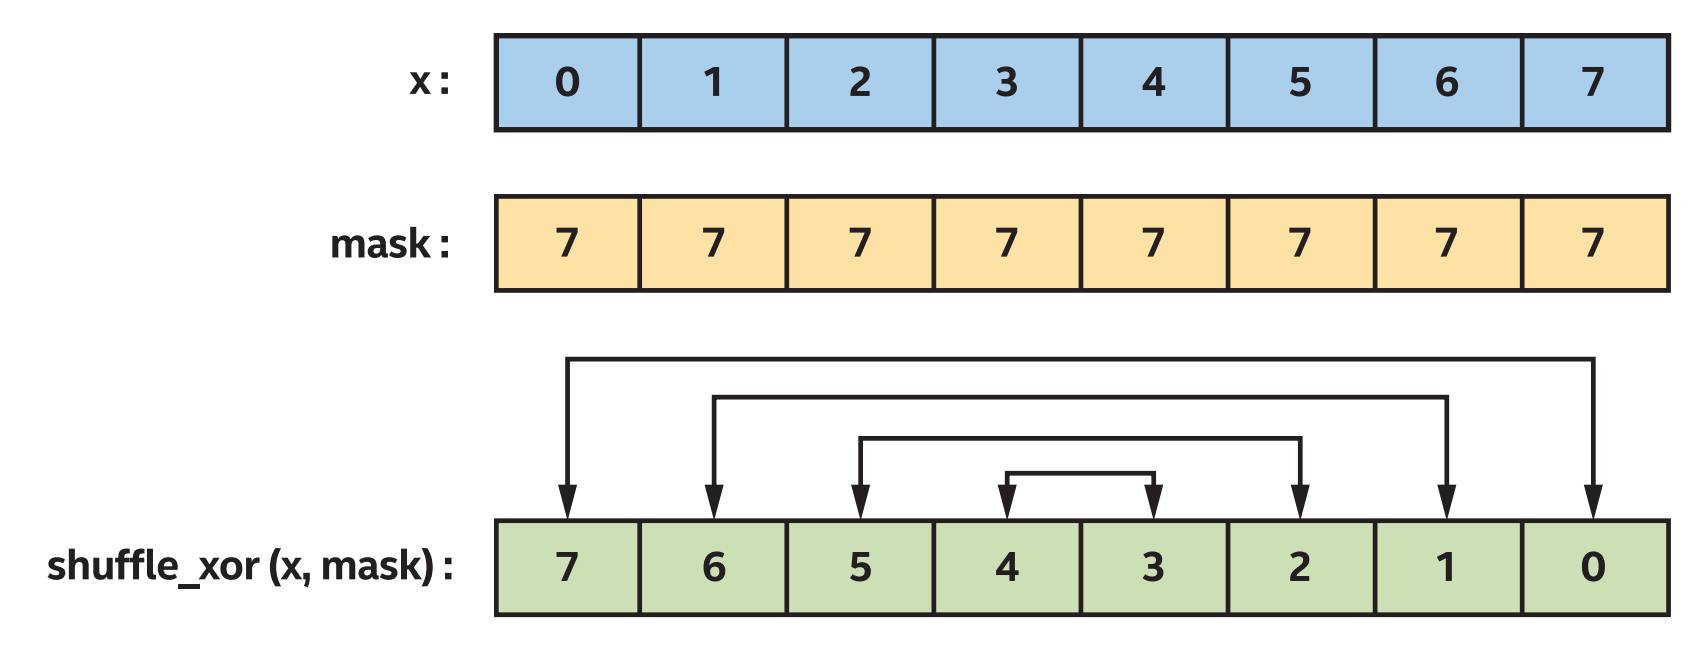
\includegraphics[width=1.\textwidth]{content/chapter-9/images/12}
\end{center}

\begin{tcolorbox}[colback=blue!5!white,colframe=blue!75!black, title=使用优化的广播,投票和集合函数]
应用于子工作组的广播、投票和其他集合函数的行为与应用于工作组的行为是相同的,但是需要注意的是,它们会在某些编译器中启用主动优化,例如:编译器可能能够减少广播到子工作组中所有工作项的变量的寄存器使用,或者能够基于any\_of和all\_of函数的使用推断出控制流的方向。
\end{tcolorbox}

\hspace*{\fill} \par %插入空行
\textbf{加载和存储}

子工作组的加载和存储函数有两个目的:第一,通知编译器子工作组中的所有工作项都从内存中的相同(统一)位置加载连续数据;第二,能够请求优化的加载/存储大量连续数据。\par

对于ND-Range parallel\_for,编译器可能不清楚由不同工作项计算的地址如何关联。例如,如图9-20所示,从每个工作项的角度来看,从索引[0,32)访问一个连续的内存块似乎是跨越的访问模式。\par

\hspace*{\fill} \par %插入空行
图9-20 一个子工作组访问四个连续块的内存
\begin{center}
	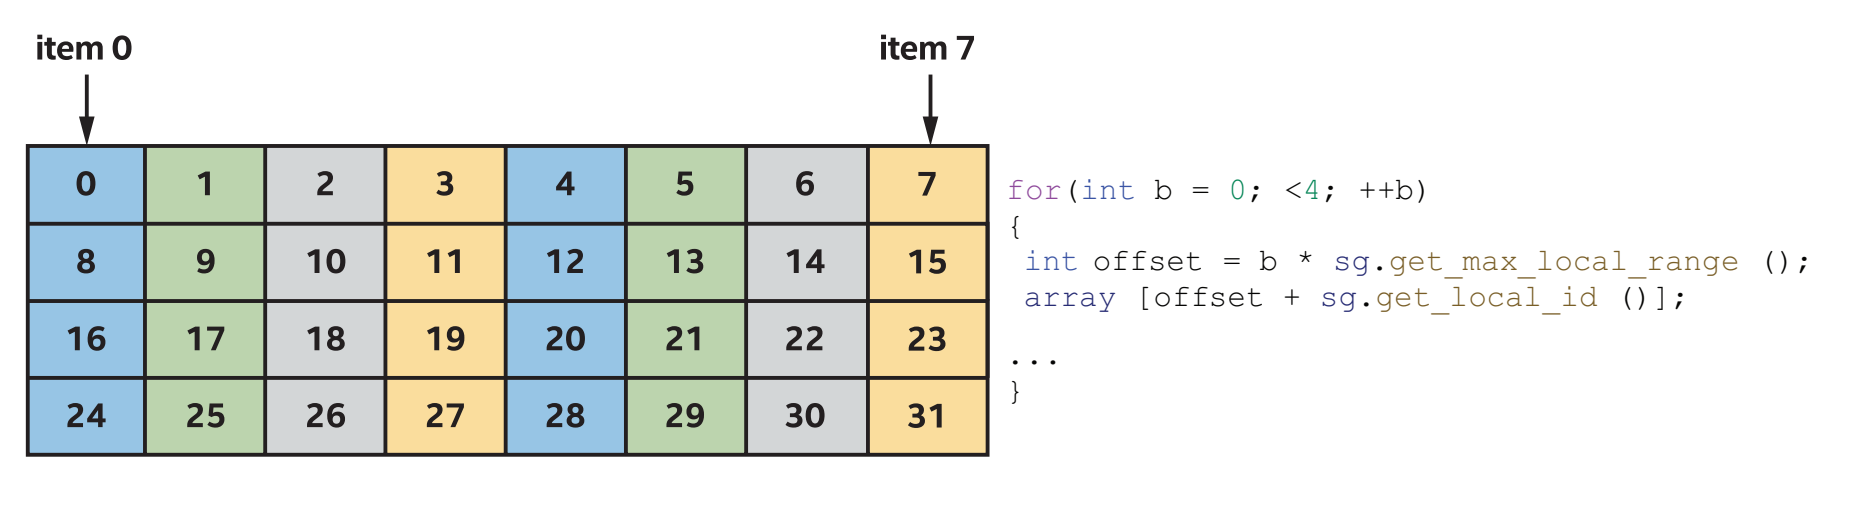
\includegraphics[width=1.\textwidth]{content/chapter-9/images/13}
\end{center}

有些体系结构包括专用硬件,用于检测子工作组中的工作项,何时访问连续数据并组合内存请求,而其他体系结构要求提前知道这一点并将其编码到加载/存储指令中。子工作组的加载和存储在任何平台上,都不是为了正确性存在的,但在某些平台上可能会提高性能,应视为一种优化提示。\par

































